% !TEX root = ../../main.tex


\begin{figure}[p]
\centering
\vspace*{-5pt}
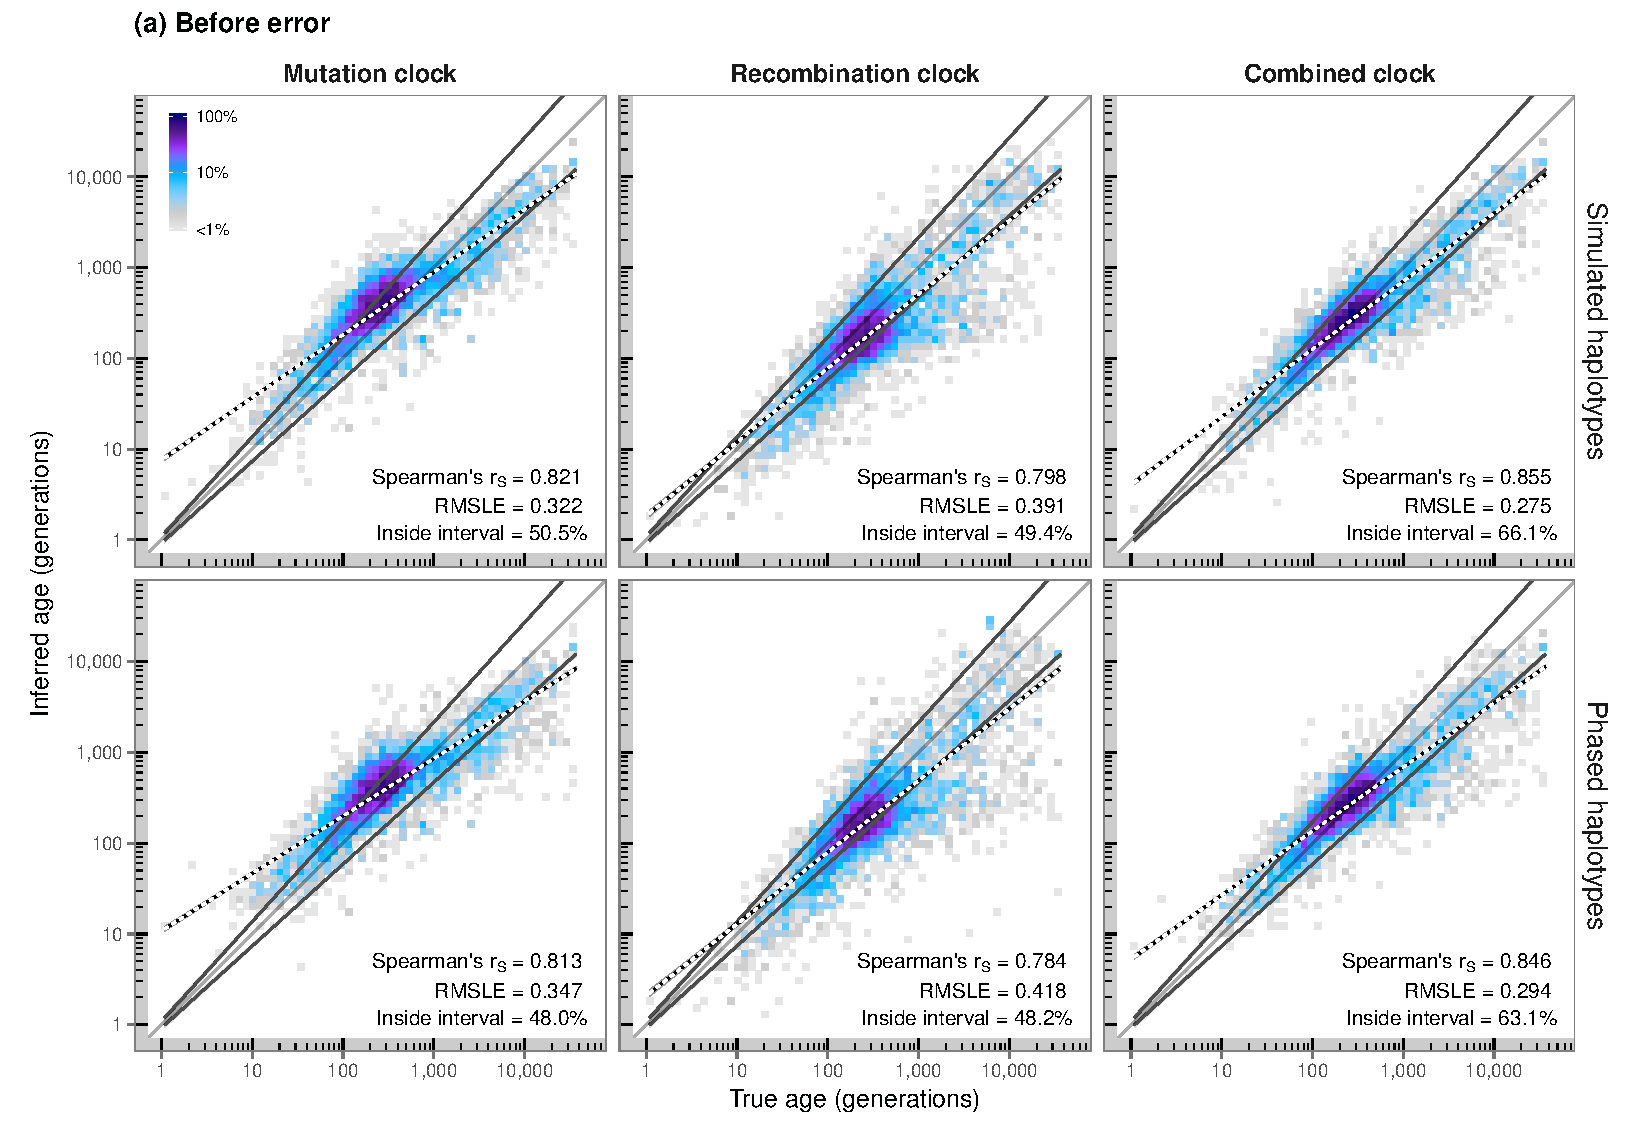
\includegraphics[width=0.95\textwidth]{./img/ch5/hhmm_age_A}
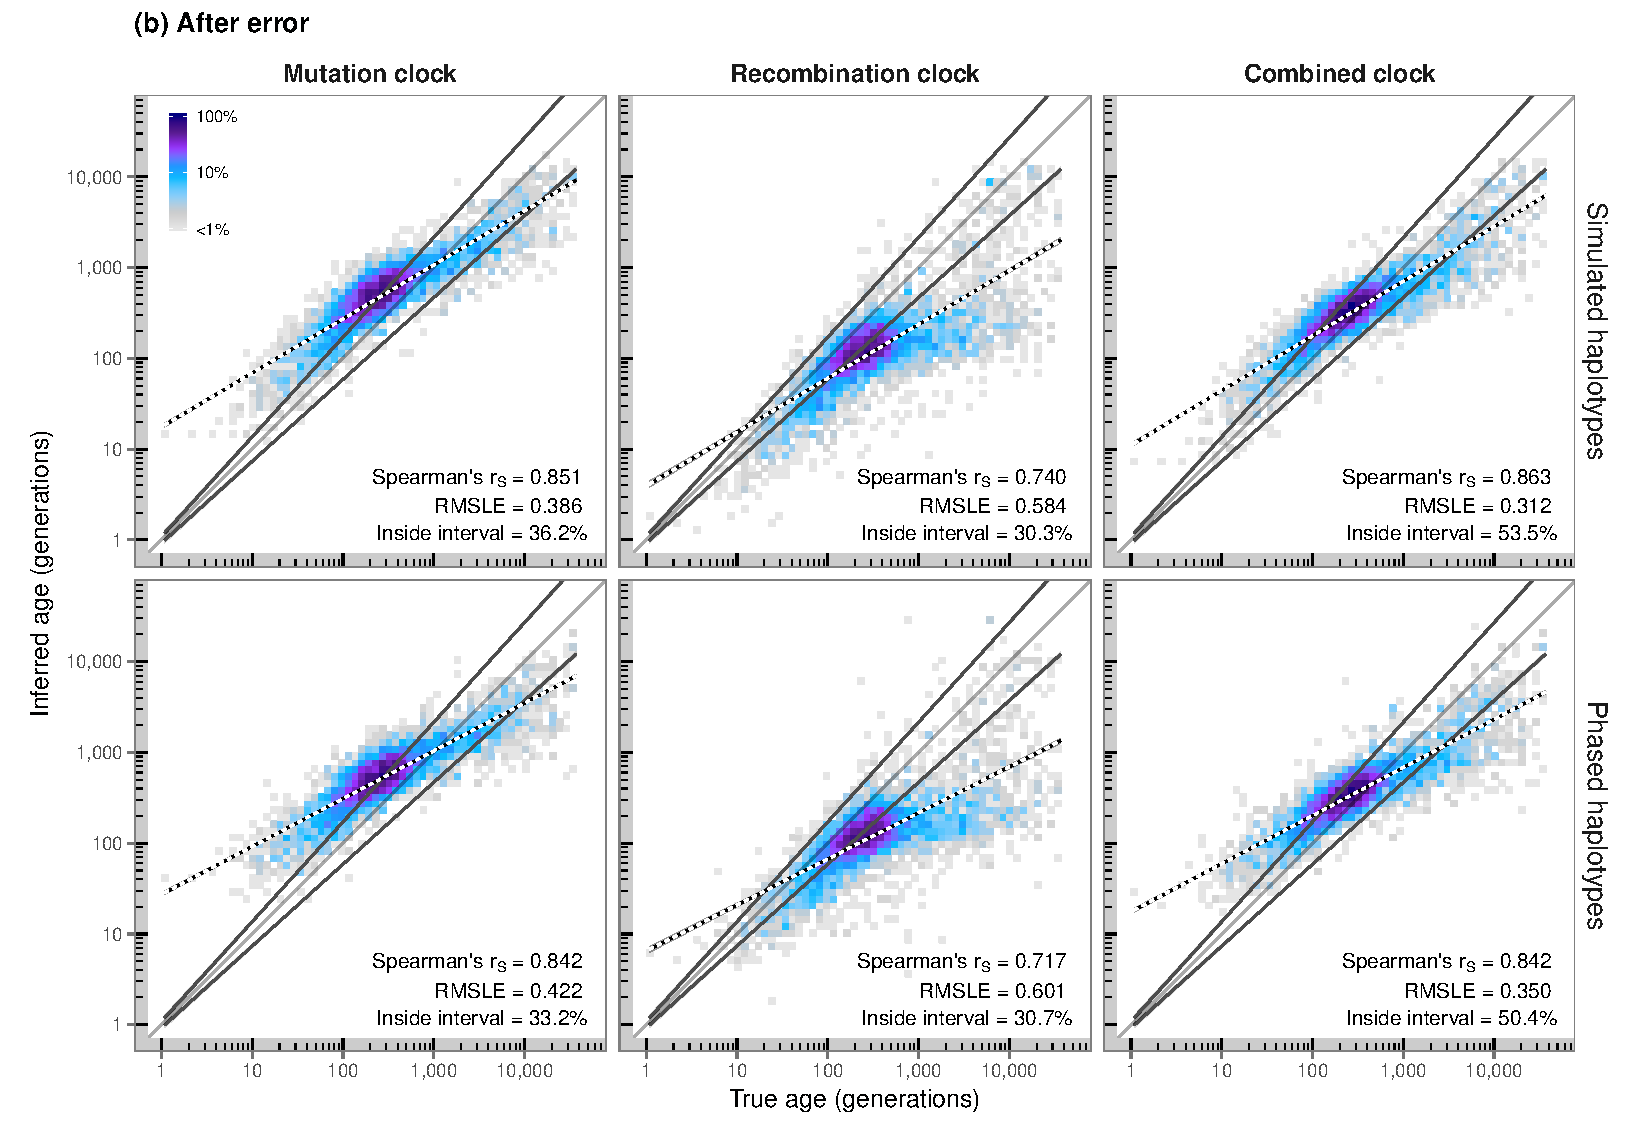
\includegraphics[width=0.95\textwidth]{./img/ch5/hhmm_age_B}
\Caption{Allele age inferred using the haplotype-based HMM}
{The haplotype-based \gls{hmm} was used to infer breakpoint intervals in data before \textbf{(a)} and after error \textbf{(b)}; analyses were conducted on ``true'' (simulated) haplotypes and phased haplotypes.
Age was estimated using each of the \n{3} clock models, for a random set of \n{5000} target sites at \fk{2,50}, for which \n{100} concordant pairs were randomly selected and \n{100} discordant pairs were selected using the relaxed nearest neighbour approach.
Note that ``true'' age was set at $t_m$, according to which the summary metrics shown were calculated.
Regression lines above and below the dividing line indicate $t_c$ and $t_d$.
The \emph{black-white} line shows the regression over age estimates.
Colours indicate the density of true and estimated age; scaled as the maximised density per panel.}
{fig:hhmm_age}
\end{figure}
